
\documentclass[twoside,a4paper,12pt]{report}
\usepackage{graphicx}
\usepackage{amsmath}
\usepackage{appendix}
\usepackage{nameref}
\usepackage{url}
\def\UrlBreaks{\do\/\do-}
\Urlmuskip=0mu plus 1mu
\usepackage[
backend=biber,
style=alphabetic
]{biblatex}
\setcounter{biburllcpenalty}{7000}
\setcounter{biburlucpenalty}{8000}
 \usepackage[T1]{fontenc} 
 \usepackage[final]{microtype}
\emergencystretch=1em
\graphicspath{ {images/} }
\usepackage[utf8]{inputenc}
\usepackage[spanish,english]{babel}



\usepackage{titlesec}

\setcounter{secnumdepth}{4}

\titleformat{\paragraph}
{\normalfont\normalsize\bfseries}{\theparagraph}{1em}{}
\titlespacing*{\paragraph}
{0pt}{3.25ex plus 1ex minus .2ex}{1.5ex plus .2ex}
 
\setlength{\parindent}{4em}
\setlength{\parskip}{1em}
\renewcommand{\baselinestretch}{1.3}

\usepackage{indentfirst}

\usepackage{mathptmx}


\usepackage{listings}
\usepackage{xcolor}
 
\definecolor{codegreen}{rgb}{0,0.6,0}
\definecolor{codegray}{rgb}{0.5,0.5,0.5}
\definecolor{codepurple}{rgb}{0.58,0,0.82}
\definecolor{backcolour}{rgb}{0.95,0.95,0.92}
 
\lstdefinestyle{mystyle}{
    backgroundcolor=\color{backcolour},   
    commentstyle=\color{codegreen},
    keywordstyle=\color{magenta},
    numberstyle=\tiny\color{codegray},
    stringstyle=\color{codepurple},
    basicstyle=\ttfamily\footnotesize,
    breakatwhitespace=false,         
    breaklines=true,                 
    captionpos=b,                    
    keepspaces=true,                 
    numbers=left,                    
    numbersep=5pt,                  
    showspaces=false,                
    showstringspaces=false,
    showtabs=false,                  
    tabsize=2
}
 
\lstset{style=mystyle}



\graphicspath{ {images/} }

\usepackage[]{geometry}
 \geometry{
 a4paper,
 total={170mm,257mm},
 inner=25mm,
 outer=25mm,
 top=25mm,
 bottom=25mm
 }
 
 



\usepackage{csquotes}

\addbibresource{references.bib}

\usepackage{titlesec}

\titleformat{\paragraph}
{\normalfont\normalsize\bfseries}{\theparagraph}{1em}{}
\titlespacing*{\paragraph}
{0pt}{3.25ex plus 1ex minus .2ex}{1.5ex plus .2ex}
 
\setlength{\parindent}{4em}
\setlength{\parskip}{1em}
\renewcommand{\baselinestretch}{1.3}

\usepackage{indentfirst}

\usepackage[]{geometry}
 \geometry{
 a4paper,
 total={170mm,257mm},
 inner=25mm,
 outer=25mm,
 top=25mm,
 bottom=25mm
 }
 
% \title{Machine learning and pattern recognition project}
\usepackage{csquotes}
\begin{document}

\tableofcontents

\newpage


\setcounter{chapter}{1}


\section{Dataset}

The dataset contains the information of red and white variants of the Portuguese "Vinho Verde" wine. It has been splitted into Test and Train sets containing 1822 and 1839 samples respectively. Moreover, there are two classes: good quality (value 1) and bad quality wine (value 0), where each has twelve attributes: 

DISTRIBUTION OF EACH ATTRIBUTES AND RANGE

\begin{itemize}
    \item fixed acidity
    \item volatile acidity
    \item citric acid
    \item residual sugar
    \item chlorides
    \item free sulfur dioxide
    \item total sulfur dioxide
    \item density
    \item pH
    \item sulphates
    \item alcohol
\end{itemize}


\subsection{Range and distribution}

\begin{table}
\centering
 \begin{tabular}{||c c c||} 
 \hline \hline
 \makecell{Attributes} & \makecell{Range} & \makecell{Type }\\ 
 \hline\hline
 Fixed acidity & [3 ; 15.9] & Continuous\\ 
 \hline
 Volatile acidity & [0.1 ; 1.58] & Continuous\\
 \hline
 Citric acid & [0 ; 1] & Continuous \\
  \hline
 Residual sugar & [0.7 ; 23.5] & Continuous \\
  \hline
 Citric acid & [0 ; 1] & Continuous \\
 \hline
 Chlorides & [0.013 ; 0.611] & Continuous \\
 \hline
 Free sulfur dioxide & [2 ; 289] & Continuous \\
 \hline
 Total sulfur dioxide & [7 ; 440] & Continuous \\
  \hline
 Density & [0.9874 ; 1.0032] & Continuous \\
  \hline
  pH & [2.79 ; 3.9 ] & Continuous \\
   \hline
 Sulphates & [0.25 ; 1.36] & Continuous \\
  \hline
 Alcohol & [8 ; 14.9] & Continuous \\
  \hline
 Total sulfur dioxide & [7,440] & Continuous \\
 \hline \hline
\end{tabular}
\label{RangeAndTypesAttributes}
\caption{Range and types of the attributes}
\end{table}


histograms figure \ref{HistogramsWithoutMod} 
\begin{figure}
    \centering
    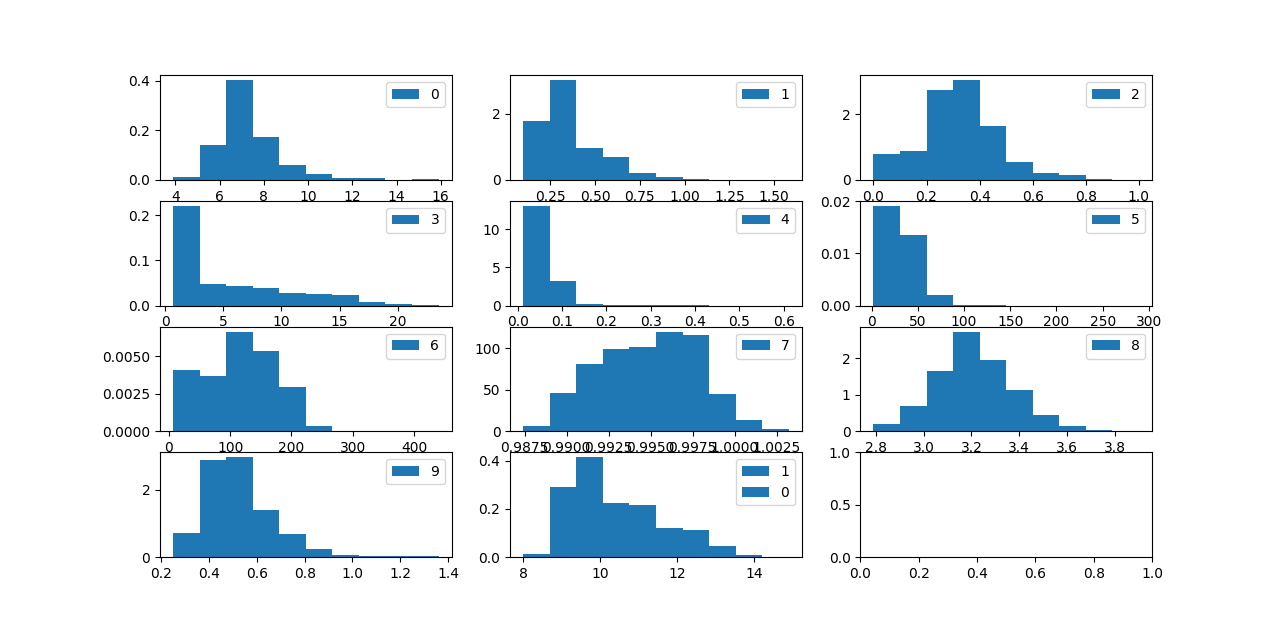
\includegraphics[width=1\textwidth,height=0.7\textheight]{histograms.png}
    \caption{Histograms of the attributes (numerated) without modification}
     \label{HistogramsWithoutMod} 
\end{figure}






\section{Classifiers}

\subsection{Without previous analysis}

In order to classify the data, different models have been taken into account : mutlivariate gaussian classifier, tied covariance, Naive Bayes and a k-fold approach. The results are shown in the table \ref{diffTypesclass}.
\begin{table}
\centering
 \begin{tabular}{||c c||} 
 \hline \hline
 \makecell{Classifier} & \makecell{Accuracy (\%)} \\
 \hline\hline
 Multivariate & 80.46  \\ 
 \hline
 Tied Covariance & 81.44\\
 \hline
 Naive Bayes & 78.98 \\
 \hline \hline
\end{tabular}
\label{diffTypesclass}
\caption{Different types of classifiers and their accuracy}
\end{table}

The precision of the models seems to be similar, however the tied covariance model has a greater precision so far with 81.44 \% and Naive Bayes performs the worst with 78.98 \%.The explanation of the poor Naive Bayes performance can be due to the fact that when we perform the diagonalization of the covariances, we do so by putting to zero the other elements of the matrix, hence inevitably losing information. This loss of information might be the explanation of a worse performance than the other classifiers.  


\end{document}
